% !TeX root = ../cyh.tex

\chapter{实验环境与测试方法}

\section{实验环境}

% 本文采用 Linux 作为实验环境,使用 Ubuntu 20.04 作为主机操作系统,
为了验证 starry-next 内存管理模块及接口的设计与实现在 riscv64、x86\_64、loongarch64 和 aarch64 这四个架构下的正确性与性能,
我们使用了 qemu 模拟器来模拟这四个架构的运行环境,并且 qemu 模拟器的版本不应低于 8.2.0。qemu 是一个开源的虚拟机模拟器,支持多种硬件架构和操作系统,能够在主机上创建虚拟机并运行不同架构的操作系统。
同时,为了支持高版本的 qemu 模拟器,测例的本地运行都在 Ubuntu-24.04 下进行,并且需要在本地安装 rustling 工具链等 rust 相关工具,具体的操作可以参考项目的 README.md 文件。

另外,为了进行自动化测试,我们使用了 GitHub Actions 来实现自动化测试,定义了多个工作流配置文件,涵盖了不同架构和测试场景的自动化构建与验证。

测试分为功能测试和性能测试。

\section{功能测试}

\subsection{测试用例}

功能测试的测试用例分为两部分:开源测试用例和自定义测试用例。
其中开源测试用例主要来自 libc-test 库。libc-test 是一个针对 C 标准库(libc)功能及兼容性的检测工具。C 标准库作为 C 语言开发的基石,涵盖输入输出、内存管理、字符串操作等基础功能。
libc-test 借助一系列精心设计的测试用例,全面且细致地检验 C 标准库各功能模块,保障其在不同环境下的正确性和稳定性。在具体测试中,将编译完成的 libc-test 可执行文件作为输入,运行其中的静态与动态测试用例。
通过执行这些测试用例并检查输出结果,可判断待测内核是否能正确支持 C 标准库的各项功能,进而评估内核与 C 标准库的兼容性与稳定性。

尽管 libc-test 库提供了丰富的测试用例,可以涵盖大多数系统调用,例如 mmap、munmap、mprotect 等,但由于 libc-test 针对的是 C 标准库,而不是操作系统内核和系统调用的实现,
同时一部分系统调用无法使用 libc-test 进行测试,例如 sysinfo、prlimit64 等系统调用。
因此,我们还编写了一些自定义测试用例来验证 starry-next 内存管理模块的功能以及系统调用接口的正确性。这些用例将通过 C 标准库中 sys 子目录直接调用相关的系统调用,
并验证其返回值,例如:

\begin{lstlisting}[language=c, caption=prlimit64]
    #include <sys/syscall.h>
    syscall(SYS_prlimit64, getpid(), RLIMIT_STACK, NULL, &old_limit);
\end{lstlisting}

\begin{lstlisting}[language=c, caption=sysinfo]
    #include <sys/sysinfo.h>
    struct sysinfo info;
    sysinfo(&info);
\end{lstlisting}

在测例的编写和运行过程中,strace 指令可以帮助我们跟踪系统调用的执行情况,在 Ubuntu-24.04 下通过 strace 指令可以得到 x86\_64 架构下的系统调用信息,
使用 qemu 模拟器配合 strace 指令也可以得到其他架构下的系统调用信息。
这些不仅可以帮助验证测例的正确性,还可以作为对照组可以帮助我们分析 starry-next 内存管理模块的实现是否符合 Linux 的标准实现,
以及系统调用的实现的正确性,从而进行进一步的调试和优化。

\subsection{测试结果与分析}

接下来,我们将从系统调用的角度对测试结果进行展示与分析。

\subsubsection{mmap 和 munmap 系统调用}

要验证 mmap 系统调用的正确性,一方面可以通过本地使用 strace 指令在 libc-test 中找出使用了该系统调用的测试用例,例如 fdopen,这里我们展示 fdopen 测例在 x86\_64 架构下的测试结果:
\begin{lstlisting}[language=bash, caption=fdopen 测试结果]
    ========== START entry-static.exe fdopen ==========
    ...
    [  1.836930 1:11 starry::syscall:12] Syscall mmap
    [  1.838002 1:11 starry_api::imp::mm::mmap:100] mmap: addr: 0x0, length: 1000, prot: MmapProt(PROT_READ | PROT_WRITE), flags: MmapFlags(MAP_PRIVATE | MAP_ANONYMOUS), fd0
    [  1.845482 1:11 starry::syscall:145] Syscall mmap return 4096
    ...
    [  2.024200 1:11 starry::syscall:12] Syscall munmap
    [  2.027765 1:11 starry::syscall:145] Syscall munmap return 0
    ...
    Pass!
    ========== END entry-static.exe fdopen ==========
\end{lstlisting}

从结果中可以看到,fdopen 测试用例执行了 mmap 系统调用,创建一个长度为 1000 字节的匿名私有映射,这段内存区域可以被读取和写入。返回值为 4096,说明系统自动选择的起始地址是 0x1000,映射成功。
并且测例整体也是通过的,说明 mmap 系统调用匿名映射部分的实现是正确的。而 munmap 系统调用的返回值为 0,说明解除映射成功。

另一方面,我们还可以通过自定义测试用例来验证 mmap 系统调用的正确性,例如:
\begin{lstlisting}[language=c, caption=自定义 mmap 测试用例]
    fd = open("test_mmap.txt", O_RDWR | O_CREATE);
    array = mmap(NULL, kst.st_size, PROT_WRITE | PROT_READ, MAP_FILE | MAP_SHARED, fd, 0);
    printf("mmap content: %s\n", array);
\end{lstlisting}

在这个测试用例中,我们打开了一个文件,并使用 mmap 系统调用将该文件映射到内存中,然后读取文件内容并打印出来。
从运行结果来看,内核成功地将文件映射到内存中,并且可以正确读取文件内容,说明 mmap 系统调用的实现是正确的。

\begin{lstlisting}[language=bash, caption=自定义 mmap 测试用例结果]
========== START test_mmap ==========
file len: 27
mmap content:   Hello, mmap successfully!
========== END test_mmap ==========
\end{lstlisting}

\subsubsection{brk 系统调用}

brk 系统调用用于设置进程的堆空间的结束地址,因而要验证 brk 系统调用的正确性,可以通过反复设置和获取堆空间的结束地址来验证其实现是否正确。
例如 libc-test 中的 mbc 测试用例,在 x86\_64 架构下的测试结果如下: 
\begin{lstlisting}[language=c, caption=brk]
    [  1.817163 1:11 starry::syscall:12] Syscall brk
    [  1.819303 1:11 starry::syscall:145] Syscall brk return 1073741824
    [  1.821880 1:11 starry::syscall:12] Syscall brk
    [  1.823235 1:11 starry::syscall:145] Syscall brk return 1073750016
\end{lstlisting}

从结果中可以看到,brk 系统调用的返回值是 1073741824 和 1073750016,分别表示堆空间的结束地址是 1GB 和 1.5GB。
这说明 brk 系统调用的实现是正确的。

\subsubsection{sysinfo 和 prlimit64 系统调用}

sysinfo 和 prlimit64 系统调用的自定义测试用例主要是通过获取系统信息和进程限制来验证其实现是否正确。在 riscv64 架构下的测试结果如下:

\begin{figure}
    \centering
    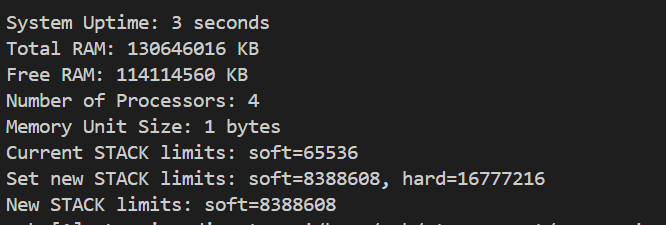
\includegraphics[width=0.5\linewidth]{sysinfo.png}
    \caption{sysinfo 和 prlimit64 测试结果}
    \label{fig:sysinfo-test}
\end{figure}

从图\ref{fig:sysinfo-test}中可以看到,sysinfo 系统调用返回了系统的内存使用情况,包括总内存和空闲内存等信息,并且 prlimit64 系统调用返回了进程用户栈的限制信息。
同时,当设置用户栈大小时,prlimit64 系统调用正确使用了新的软限制值,
这说明 sysinfo 和 prlimit64 系统调用用户栈选项的功能正常。而 prlimit64 的最大文件数量限制则可以通过 libc-test 的 rlimit\_open\_files 测试用例来验证,
该测例会在设置资源限制后重复创建新的文件描述符(打开文件)至失败,并取当前最大文件描述符和资源限制值进行比较,相等则说明实现正确。该测例也是通过的。

\begin{figure}
    \centering
    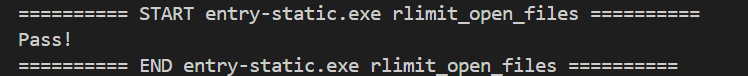
\includegraphics[width=0.5\linewidth]{prlimit64.png}
    \caption{rlimit\_open\_files 测例结果}
    \label{fig:prlimit64-test}
\end{figure}

\section{性能测试}

当前并未对 starry-next 内存管理模块的性能进行专项测试,
但在功能测试中,部分测例的运行时间也可以作为性能测试的参考。我们将 starry-next 内存管理模块的性能与 Linux 的标准实现进行对比,
以验证 starry-next 内存管理模块的性能是否符合 Linux 的标准实现。

以功能测试中的自定义 mmap 测试用例为例,
在 x86\_64 架构下的测试结果如下:
\begin{figure}[H]
    \centering  % 图片全局居中
    \begin{subfigure}[t]{0.45\textwidth}
        \centering
        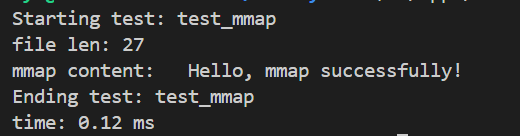
\includegraphics[width=\linewidth]{s2-local.png}
        \caption{Linux}
        \label{fig:sub.1}
    \end{subfigure}
    \hfill % 添加一些水平间距
    \begin{subfigure}[t]{0.45\textwidth}
        \centering
        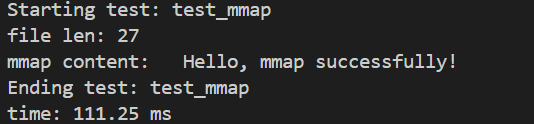
\includegraphics[width=\linewidth]{s2-starry.png}
        \caption{starry-next}
        \label{fig:sub.2}
    \end{subfigure}
    \caption{自定义 mmap 测试用例的运行时间对比}
    \label{Fig.main}
\end{figure}

不难看出,starry-next 花费的时间远高于本机的运行时间。为了减少其他模块的影响,
本文还设计了一个简单的 c 程序,该程序重复进行系统调用,
并将其运行时间与 Linux 的标准实现进行对比,
结果如下:

\begin{figure}[H]
    \centering  % 图片全局居中
    \begin{subfigure}[t]{0.45\textwidth}
        \centering
        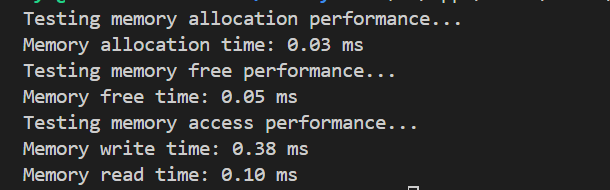
\includegraphics[width=\linewidth]{s1.png}
        \caption{Linux}
        \label{fig:sub.3}
    \end{subfigure}
    \hfill % 添加一些水平间距
    \begin{subfigure}[t]{0.45\textwidth}
        \centering
        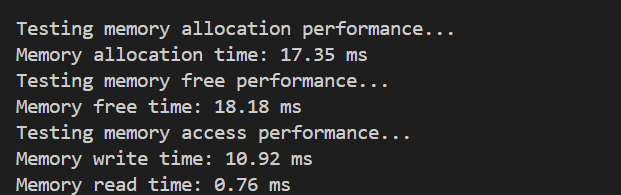
\includegraphics[width=\linewidth]{s1-starry.png}
        \caption{starry-next}
        \label{fig:sub.4}
    \end{subfigure}
    \caption{重复进行系统调用的运行时间对比}
    \label{Fig.main2}
\end{figure}

由图\ref{Fig.main2}可见starry-next 在映射、解除映射、读取和写入数据等方面花费的时间远高于本机的运行时间,
尽管 starry-next 的运行还要受到 qemu 模拟器的影响,自身也实现了 Lazy Map 等内存管理方面的优化机制,
但总体来说,其性能仍有很大的提升空间。